\section{Schedulering}

\begin{figure}[h!]
	\centering
	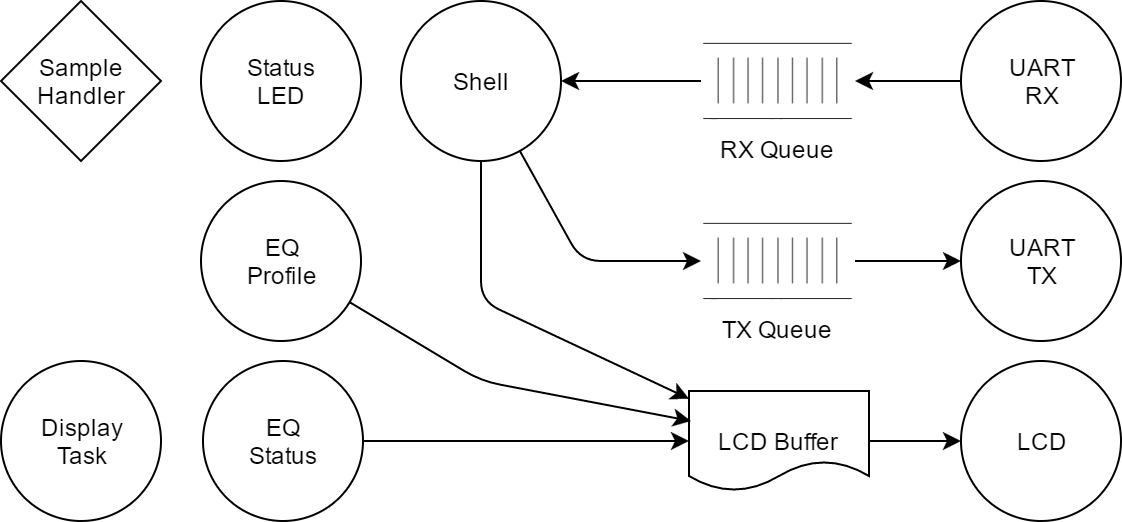
\includegraphics[width=.7\textwidth]{billeder/eq-one.png}
	\caption{Task model af equalizerens operativ system.}
	\label{fig:eq-taskmodel}
\end{figure}

Det er valgt at bruge en variant af RTCS (Run To Completion Scheduler)\footnote{RTCS blev introduceret i faget embedded programmering.}. 
Den valgte model for task schedulering er ikke preemtive, således vil task der bliver sat i kø til udførelse forblive aktive indtil de afslutter sig selv.
\textbf{sysTick} tiden for scheduleringen er sat til $1\si{\milli\second}$.\\

I figur \ref{fig:eq-taskmodel} ses task modellen for equalizeren. 
Der er i hele systemet ikke brugt semaphore beskyttelse af \textit{queues} eller buffere, da oprativ systemet er ikke preemtive. \\

Alle task der er klar til at blive behandlet af scheduleren, bliver det i den rækkefølge de er oprettet og ligger i \textbf{task pool}. 
I figur \ref{fig:eq-taskstates} ses state diagrammet over de tilstande en task kan befinde sig i.
Ud over at scheduleringen forgår sekventielt, er hver task tilknyttet en tidsprioritet. 
Således vil en task kunne have prioritet lav = 10, mellem = 5 og høj = 1, som angiver hvor mange \textbf{sysTick}'s af schedulere før de kommer til.
I figur \ref{fig:eq-sched-algo} ses shedulerings algoritmen.

\begin{figure}[h]
	\centering
	\subbottom[]{%
		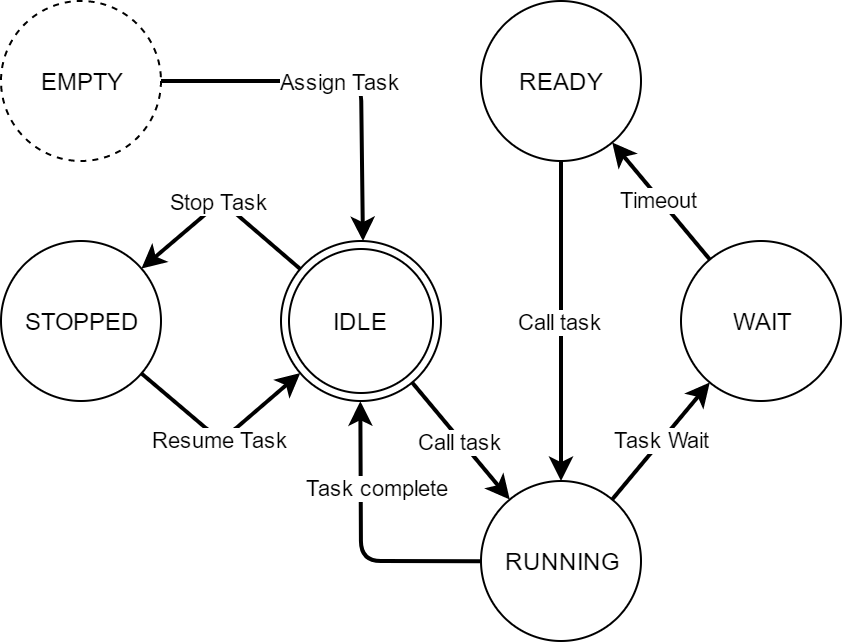
\includegraphics[width=0.48\textwidth]{billeder/task_states.png}
		\label{fig:eq-taskstates}}
	\subbottom[]{%
		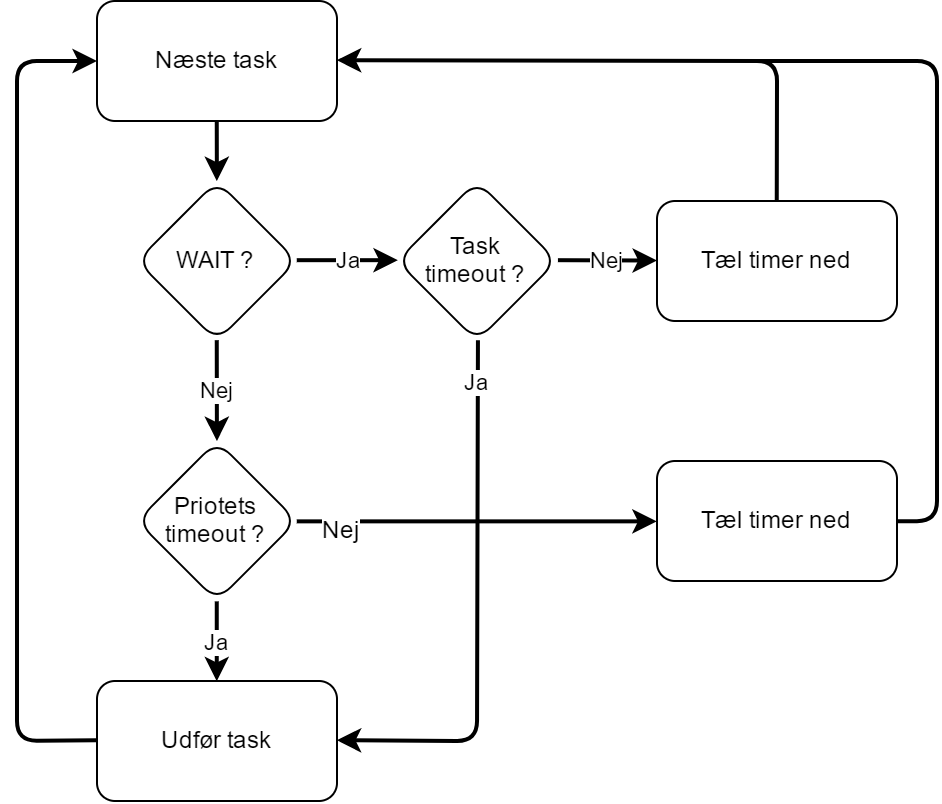
\includegraphics[width=0.48\textwidth]{billeder/scheduler_algoritme.png}
		\label{fig:eq-sched-algo}}
	\caption{(a) Task state diagram der bruges af scheduleren. (b) Scheduler algoritme}
\end{figure}
\FloatBlock

%\begin{figure}[h!]
%	\centering
%	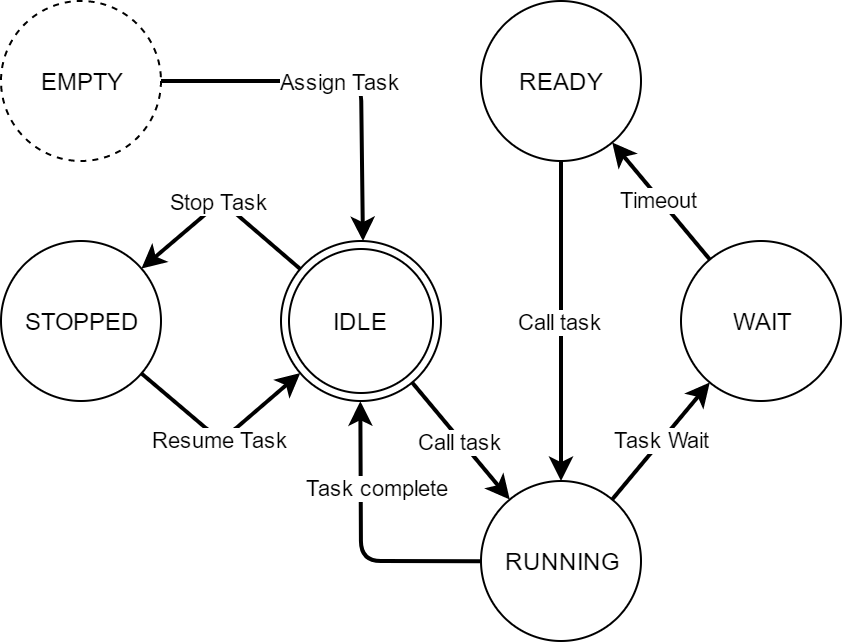
\includegraphics[width=.5\textwidth]{billeder/task_states.png}
%	\caption{Task state diagram der bruges af scheduleren.}
%	\label{fig:eq-taskstates}
%\end{figure}
%
%\begin{figure}[h!]
%	\centering
%	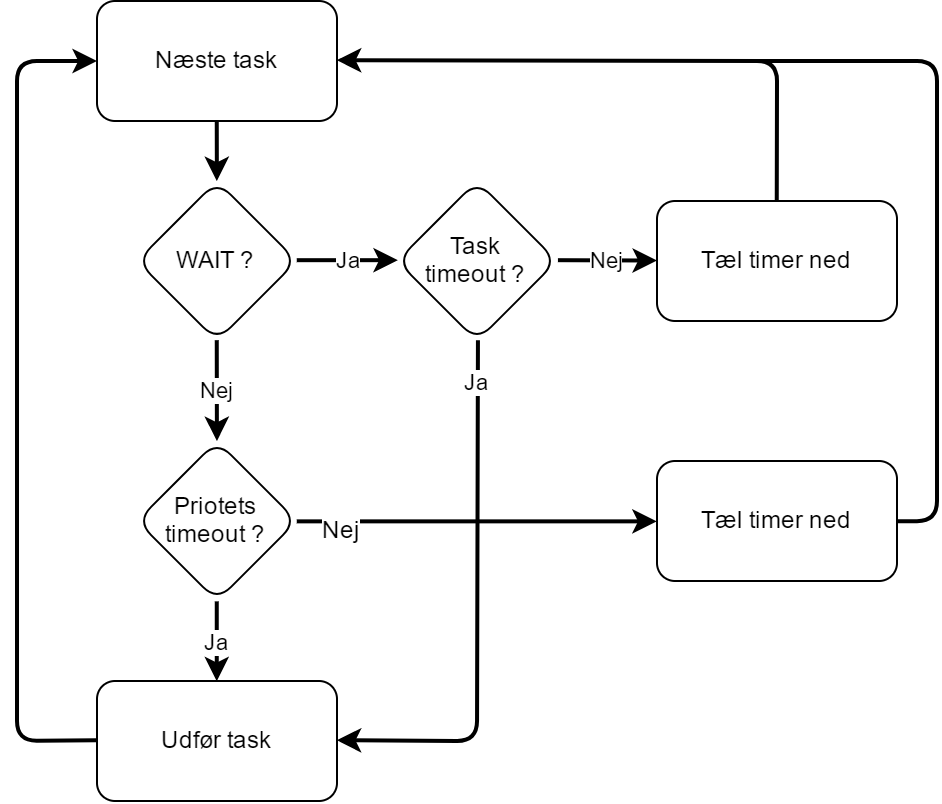
\includegraphics[width=.5\textwidth]{billeder/scheduler_algoritme.png}
%	\caption{.}
%	\label{fig:eq-sched-algo}
%\end{figure}



%Task diagram af interrupt vs. schedulering.
%Forklar (diagram) algoritmen for scheduleringen. Prioritet af tasks, etc.
%State diagram af schedulering.
%Argumentere og for at systicks ikke misses pga. int. prioritering og at sceduleringen kan tage højde for dette.
%Overbevis læseren om at scheduleringen er effektiv til formålet .
%Noter:
%Problemer med schedulring når der ikke er tid til de enkelt tasks inden for et tick, når eq bliver aktiveret bliver der endnu mindre tid og så sker det at der misses ticks.
%Tag tider når OS starter op uden EQ tændt, og sammenlign med tider når EQ kører, så er tiden hver task er om at kører inkl. den tid som audio int. bruger -> nu skrider hele scheduleringen og tick misses. Især når eq-profil-amp funktionen bruges, som tager meget lang tid.
%
%Optimalt at flytte eq-profil dannelsen ind i boot sec. så den ikke bruger tid i realtime.
%
%Tiderne på LOW, MEDIUM og HIGH prioritet har indflydelse på systemet, absolut ikke den bedste løsning, en preemptive schedulering ville helt klart afhjælpe nogle af de problemer.




 

